\chapter{THỰC NGHIỆM VÀ ĐÁNH GIÁ KẾT QUẢ}
\label{chap:chuong4}

\section{Môi trường thực nghiệm và thiết lập kiểm thử}
\label{sec:moi-truong-thuc-nghiem}

Toàn bộ các thực nghiệm trong đề tài được tiến hành trên môi trường phần cứng máy tính cá nhân đồng nhất, sử dụng hệ điều hành Windows 11 x64. Môi trường phần mềm và các gói thư viện khoa học dữ liệu mã nguồn mở được chuẩn hóa bao gồm:
\begin{itemize}
    \item Ngôn ngữ lập trình: Python phiên bản 3.10+;
    \item Thư viện học máy cốt lõi: \texttt{scikit-learn} (phiên bản $\ge 1.3.0$);
    \item Thư viện xử lý và cấu trúc dữ liệu: \texttt{pandas} ($\ge 2.0.0$), \texttt{numpy} ($\ge 1.24.0$);
    \item Thư viện trực quan hóa và đồ họa: \texttt{matplotlib} ($\ge 3.7.0$), \texttt{seaborn} ($\ge 0.12.0$);
    \item Thư viện tuần tự hóa mô hình và bộ nhớ đệm: \texttt{joblib} ($\ge 1.3.0$);
    \item Thư viện xây dựng giao diện ứng dụng web: \texttt{streamlit} ($\ge 1.30.0$).
\end{itemize}

Về thiết lập phân chia dữ liệu, như đã trình bày tại Mục~\ref{sec:kiem-soat-leakage}, tập dữ liệu sạch gồm 5.171 mẫu được phân tách theo tỷ lệ 80/20 có phân tầng nhãn:
\begin{itemize}
    \item \textbf{Tập huấn luyện (Training Set):} 4.136 tin nhắn (bao gồm 3.614 tin hợp lệ và 522 tin nhắn rác, tỷ lệ spam 12,6\%);
    \item \textbf{Tập kiểm thử độc lập (Test Set):} 1.035 tin nhắn (bao gồm 904 tin hợp lệ và 131 tin nhắn rác, tỷ lệ spam 12,7\%).
    \item Giá trị mầm ngẫu nhiên \texttt{random\_state=42} được cố định trong mọi bước phân chia để đảm bảo kết quả có thể tái lập 100\%.
\end{itemize}

\section{Thiết lập phương án cơ sở (Baseline) và kết quả mốc}
\label{sec:baseline-ket-qua}

Theo yêu cầu bắt buộc tại Mục 2 trong tài liệu hướng dẫn bài tập lớn của học phần, mỗi nhóm cần xây dựng một phương án cơ sở (Baseline) làm mốc quy chiếu để đo lường giá trị thực tế của các cải tiến kỹ thuật.

Nhóm thiết lập \textbf{Phương án Baseline} với cấu hình đơn giản và tự nhiên nhất:
\begin{itemize}
    \item \textbf{Tiền xử lý:} Sử dụng luồng thô P0 (\texttt{P0\_raw} --- chỉ chuyển chữ thường và tách từ mặc định, không chuẩn hóa regex bảo toàn tín hiệu, không loại bỏ stop words).
    \item \textbf{Biểu diễn đặc trưng:} Sử dụng mô hình túi từ BoW unigram đơn thuần (\texttt{ngram\_range=(1, 1)}, \texttt{min\_df=1}).
    \item \textbf{Siêu tham số mô hình:} Sử dụng toàn bộ siêu tham số mặc định của thư viện \texttt{scikit-learn}:
    \begin{itemize}
        \item MultinomialNB: $\alpha = 1.0$, \texttt{fit\_prior=True};
        \item K-NN: $K = 5$, \texttt{metric='euclidean'}, \texttt{weights='uniform'};
        \item DecisionTree: \texttt{criterion='gini'}, \texttt{max\_depth=None} (không giới hạn độ sâu cây), \texttt{min\_samples\_leaf=1}, \texttt{random\_state=42}.
    \end{itemize}
\end{itemize}

Kết quả thực nghiệm của phương án Baseline trên tập kiểm thử độc lập (Test Set) được ghi nhận chi tiết tại Bảng~\ref{tab:ket-qua-baseline}.

\begin{table}[H]
\centering
\caption{Hiệu năng của các mô hình ở phương án Baseline trên tập kiểm thử (1.035 tin nhắn)}
\label{tab:ket-qua-baseline}
\begin{tabular}{|l|c|c|c|c|}
\hline
\textbf{Mô hình (Cấu hình Baseline)} & \textbf{Accuracy} & \textbf{Precision} & \textbf{Recall} & \textbf{F1-Score} \\
\hline
Multinomial Naive Bayes & 0,9807 & 0,9512 & 0,8931 & 0,9213 \\
\hline
K-Nearest Neighbors (K-NN) & 0,9072 & 1,0000 & 0,2672 & \textbf{0,4217} \\
\hline
Cây quyết định (Decision Tree) & 0,9691 & 0,9024 & 0,8473 & 0,8740 \\
\hline
\end{tabular}
\Nguon{Trích xuất tự động từ kết quả baseline\_results.csv}
\end{table}

\textbf{Phân tích kết quả Baseline:}
\begin{enumerate}
    \item Mô hình Multinomial Naive Bayes đạt kết quả ban đầu khá tốt với F1-score đạt $0,9213$ (Precision $95,12\%$, Recall $89,31\%$).
    \item Mô hình Cây quyết định không giới hạn độ sâu bị hiện tượng quá khớp (Overfitting), chỉ đạt F1-score $0,8740$ và Recall $84,73\%$.
    \item \textbf{Hiện tượng thất bại thảm hại của K-NN:} Mặc dù đạt Accuracy lên tới $90,72\%$ và Precision tuyệt đối $100\%$, nhưng chỉ số Recall của K-NN chỉ đạt vỏn vẹn \textbf{$26,72\%$}, dẫn tới điểm F1 tụt dốc xuống \textbf{$0,4217$}. Điều này có nghĩa là ở cấu hình mặc định, K-NN đã \textbf{bỏ sót tới gần $73,3\%$ tổng số tin nhắn rác} trong tập kiểm thử! Nguyên nhân hoàn toàn bắt nguồn từ việc áp dụng khoảng cách Euclid trên vector đếm BoW: độ dài tin nhắn không đồng đều làm sai lệch hoàn toàn khái niệm láng giềng gần nhất.
\end{enumerate}

\section{Giai đoạn 1: Đánh giá lưới 36 cấu hình với tham số mặc định}
\label{sec:giai-doan-1}

Trong Giai đoạn 1, nhóm tiến hành khảo nghiệm toàn bộ không gian kết hợp gồm 3 mô hình $\times$ 3 mức tiền xử lý $\times$ 4 phương pháp biểu diễn, tổng cộng \textbf{36 cấu hình thực nghiệm}. Tất cả các mô hình trong giai đoạn này đều được giữ ở siêu tham số mặc định và được đánh giá thông qua thẩm định chéo 5-fold Stratified CV trên tập huấn luyện (Train Set).

Kết quả điểm số F1 trung bình của lớp spam trên 5 fold CV được trực quan hóa thông qua biểu đồ nhiệt (Heatmap) tại Hình~\ref{fig:stage1-heatmaps}.

\begin{figure}[H]
    \centering
    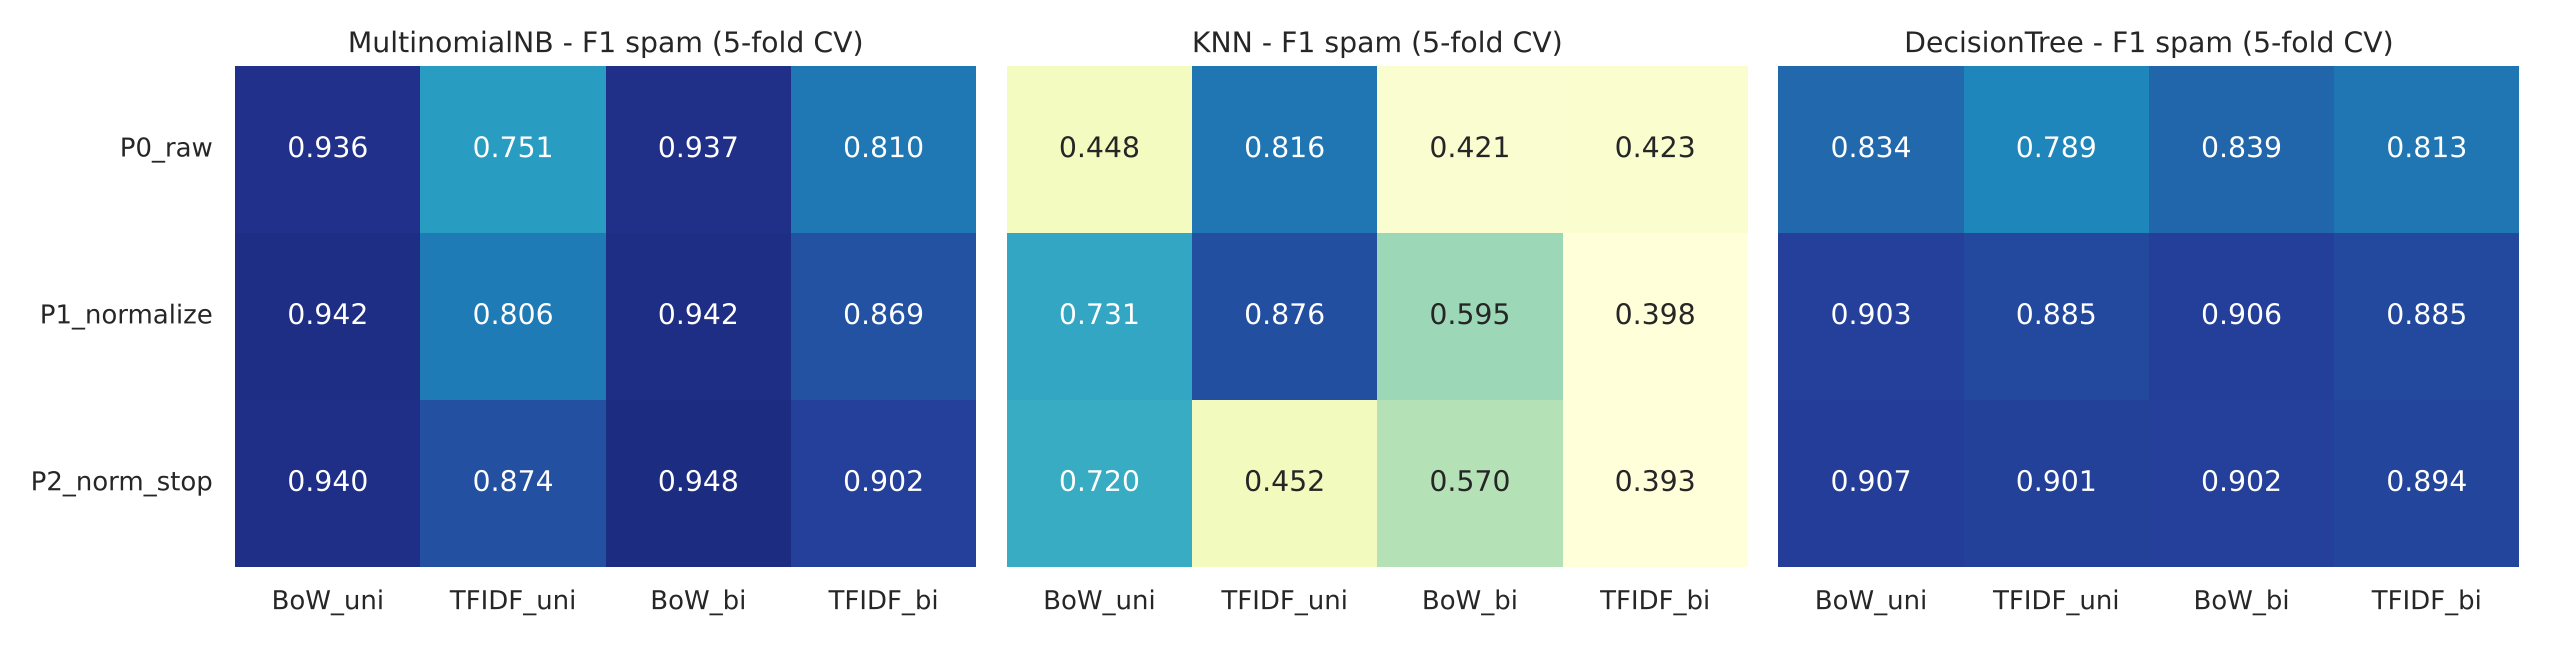
\includegraphics[width=\textwidth]{images/stage1_heatmap_cv_f1.png}
    \caption{Biểu đồ nhiệt so sánh điểm F1 lớp spam (5-fold CV) của 36 cấu hình thực nghiệm ở Giai đoạn 1 (siêu tham số mặc định)}
    \label{fig:stage1-heatmaps}
    \Nguon{Trích xuất tự động từ module run\_experiments.py}
\end{figure}

Phân tích Hình~\ref{fig:stage1-heatmaps} mang lại ba phát hiện quan trọng:
\begin{enumerate}
    \item \textbf{Tác động tích cực của tiền xử lý bảo toàn tín hiệu (P1 và P2):}
    Đối với Cây quyết định, việc chuyển từ tiền xử lý thô P0 sang P1 (bảo toàn tín hiệu regex) làm điểm F1 CV của cấu hình BoW unigram tăng vọt từ $0,834$ lên $0,903$ (tăng tới 6,9 điểm phần trăm), và tiếp tục đạt $0,907$ ở P2. Đối với Naive Bayes, F1 CV cũng tăng từ $0,936$ lên $0,942$. Điều này bước đầu kiểm chứng tính đúng đắn của Giả thuyết H1.
    \item \textbf{Nghịch lý TF-IDF trên Naive Bayes với $\alpha=1.0$ mặc định:}
    Trên biểu đồ của MultinomialNB, các ô sử dụng biểu diễn TF-IDF đều có điểm F1 rất thấp so với BoW. Cụ thể, ở mức tiền xử lý P0, BoW unigram đạt F1 là $0,936$ trong khi TF-IDF unigram chỉ đạt $0,751$ (giảm tới 18,5 điểm phần trăm). Tuy nhiên, nhóm không vội vàng kết luận TF-IDF kém hơn BoW, mà nghi vấn rằng chính hệ số làm trơn $\alpha=1.0$ mặc định đã bóp méo xác suất của các vector TF-IDF có độ lớn cực nhỏ.
    \item \textbf{Sự bất ổn định của K-NN:}
    Với khoảng cách Euclid mặc định, K-NN dao động dữ dội và có nhiều ô cấu hình F1 chỉ đạt dưới $0,400$.
\end{enumerate}

\section{Giai đoạn 2: Tinh chỉnh siêu tham số theo từng ô cấu hình}
\label{sec:giai-doan-2}

Bước sang Giai đoạn 2, nhóm triển khai kỹ thuật tinh chỉnh siêu tham số tối ưu bằng \texttt{GridSearchCV} 5-fold CV cho từng ô cấu hình của MultinomialNB và K-NN, sau đó đối sánh lại điểm F1 CV tối ưu giữa các ô.

Biểu đồ nhiệt kết quả F1 CV sau khi đã được tối ưu hóa siêu tham số được trình bày tại Hình~\ref{fig:stage2-heatmaps}.

\begin{figure}[H]
    \centering
    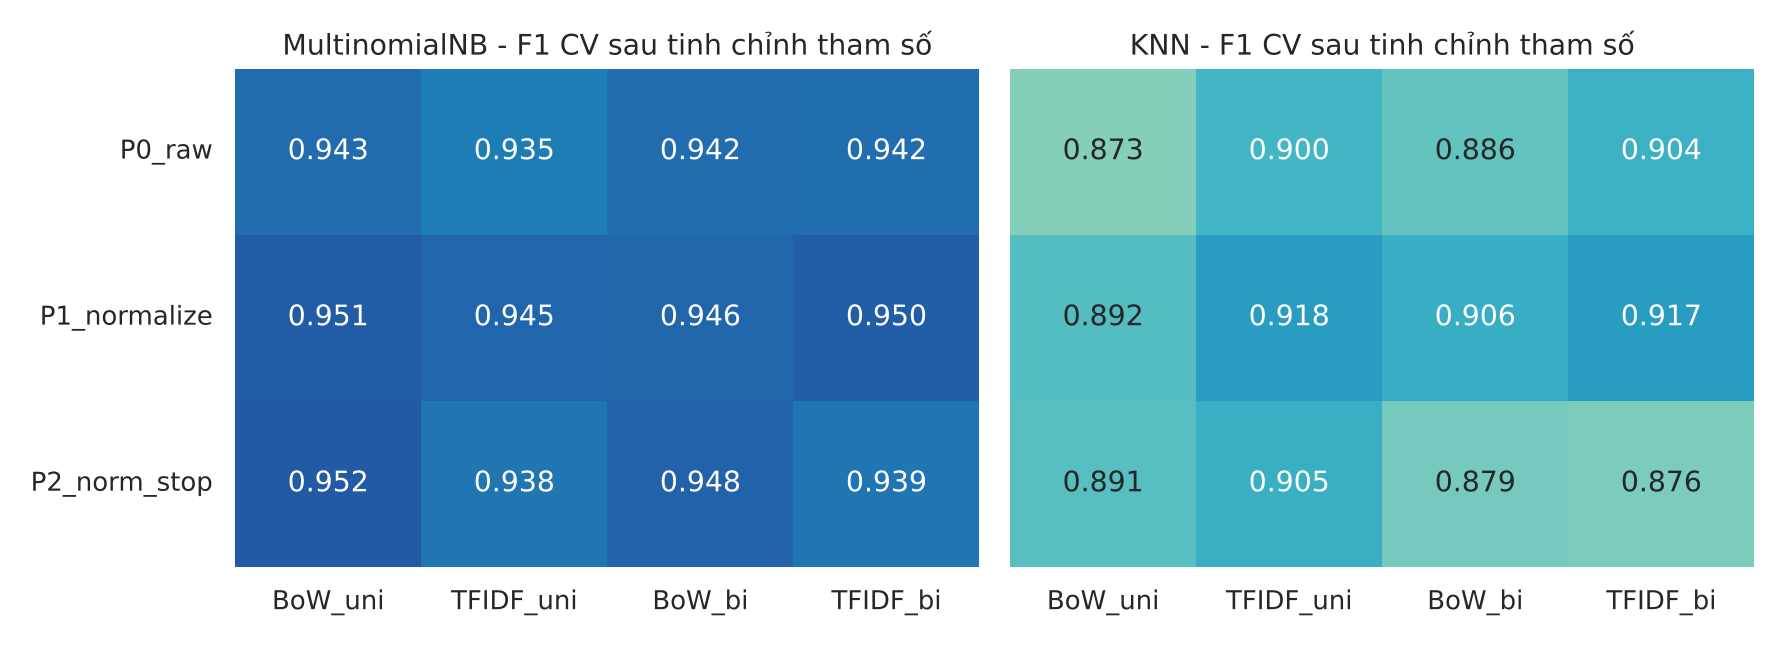
\includegraphics[width=0.88\textwidth]{images/stage2_heatmap_tuned_cv_f1.png}
    \caption{Biểu đồ nhiệt điểm F1 CV của MultinomialNB và K-NN sau khi đã tinh chỉnh siêu tham số tối ưu trong từng ô cấu hình}
    \label{fig:stage2-heatmaps}
    \Nguon{Trích xuất tự động từ module run\_experiments.py}
\end{figure}

\textbf{Phát hiện bước ngoặt từ Hình~\ref{fig:stage2-heatmaps}:}
\begin{itemize}
    \item Khi mỗi ô biểu diễn được trao cơ hội tìm kiếm siêu tham số $\alpha$ phù hợp với chính nó, khoảng cách hiệu năng giữa BoW và TF-IDF trên Naive Bayes đã \textbf{hoàn toàn biến mất}! Mọi ô cấu hình của Naive Bayes đều đạt điểm F1 CV xuất sắc trong dải rất hẹp từ $0,935$ đến $0,952$. Điều này chứng minh giả thuyết phương pháp luận của nhóm là hoàn toàn chính xác: TF-IDF ở Giai đoạn 1 bị điểm thấp thuần túy là do tham số $\alpha=1.0$ mặc định không tương thích, chứ không phải do bản chất của phép biểu diễn TF-IDF!
    \item Đối với K-NN, khi được chuyển sang khoảng cách \texttt{cosine}, trọng số \texttt{distance} và $K=9$, điểm F1 CV của cấu hình P1 + TF-IDF unigram đã tăng vọt từ $0,876$ lên \textbf{$0,918$}, đưa K-NN trở thành một bộ phân loại có hiệu năng cạnh tranh sòng phẳng với Cây quyết định.
\end{itemize}

Dựa trên kết quả F1 thẩm định chéo 5-fold CV cao nhất trên tập huấn luyện, cấu hình tối ưu cuối cùng được lựa chọn cho mỗi thuật toán được tổng hợp trong Bảng~\ref{tab:cau-hinh-toi-uu}.

\begin{table}[H]
\centering
\caption{Cấu hình tối ưu được lựa chọn cho từng mô hình dựa trên 5-fold CV tập huấn luyện}
\label{tab:cau-hinh-toi-uu}
\begin{tabular}{|l|c|c|p{4.2cm}|c|c|}
\hline
\textbf{Mô hình} & \textbf{Tiền xử lý} & \textbf{Biểu diễn} & \textbf{Siêu tham số tối ưu} & \textbf{CV-F1 mặc định} & \textbf{CV-F1 tinh chỉnh} \\
\hline
\textbf{MultinomialNB} & P2\_norm\_stop & BoW\_uni & $\alpha=2.0$, \texttt{fit\_prior=True} & 0,9400 & \textbf{0,9518} \\
\hline
\textbf{K-NN} & P1\_normalize & TFIDF\_uni & \texttt{metric='cosine'}, $K=9$, \texttt{weights='distance'} & 0,8759 & \textbf{0,9176} \\
\hline
\textbf{DecisionTree} & P2\_norm\_stop & BoW\_uni & \texttt{criterion='gini'}, \texttt{max\_depth=10}, \texttt{min\_samples\_leaf=1} & 0,9072 & \textbf{0,9110} \\
\hline
\end{tabular}
\Nguon{Trích xuất tự động từ results/summary.json}
\end{table}

\subsection{Phân tích đường cong siêu tham số}
Hình~\ref{fig:param-curves} mô tả trực quan sự biến thiên của điểm F1 CV theo các siêu tham số đơn lẻ quan trọng nhất của từng mô hình (khi các tham số còn lại được cố định tại giá trị tối ưu).

\begin{figure}[H]
    \centering
    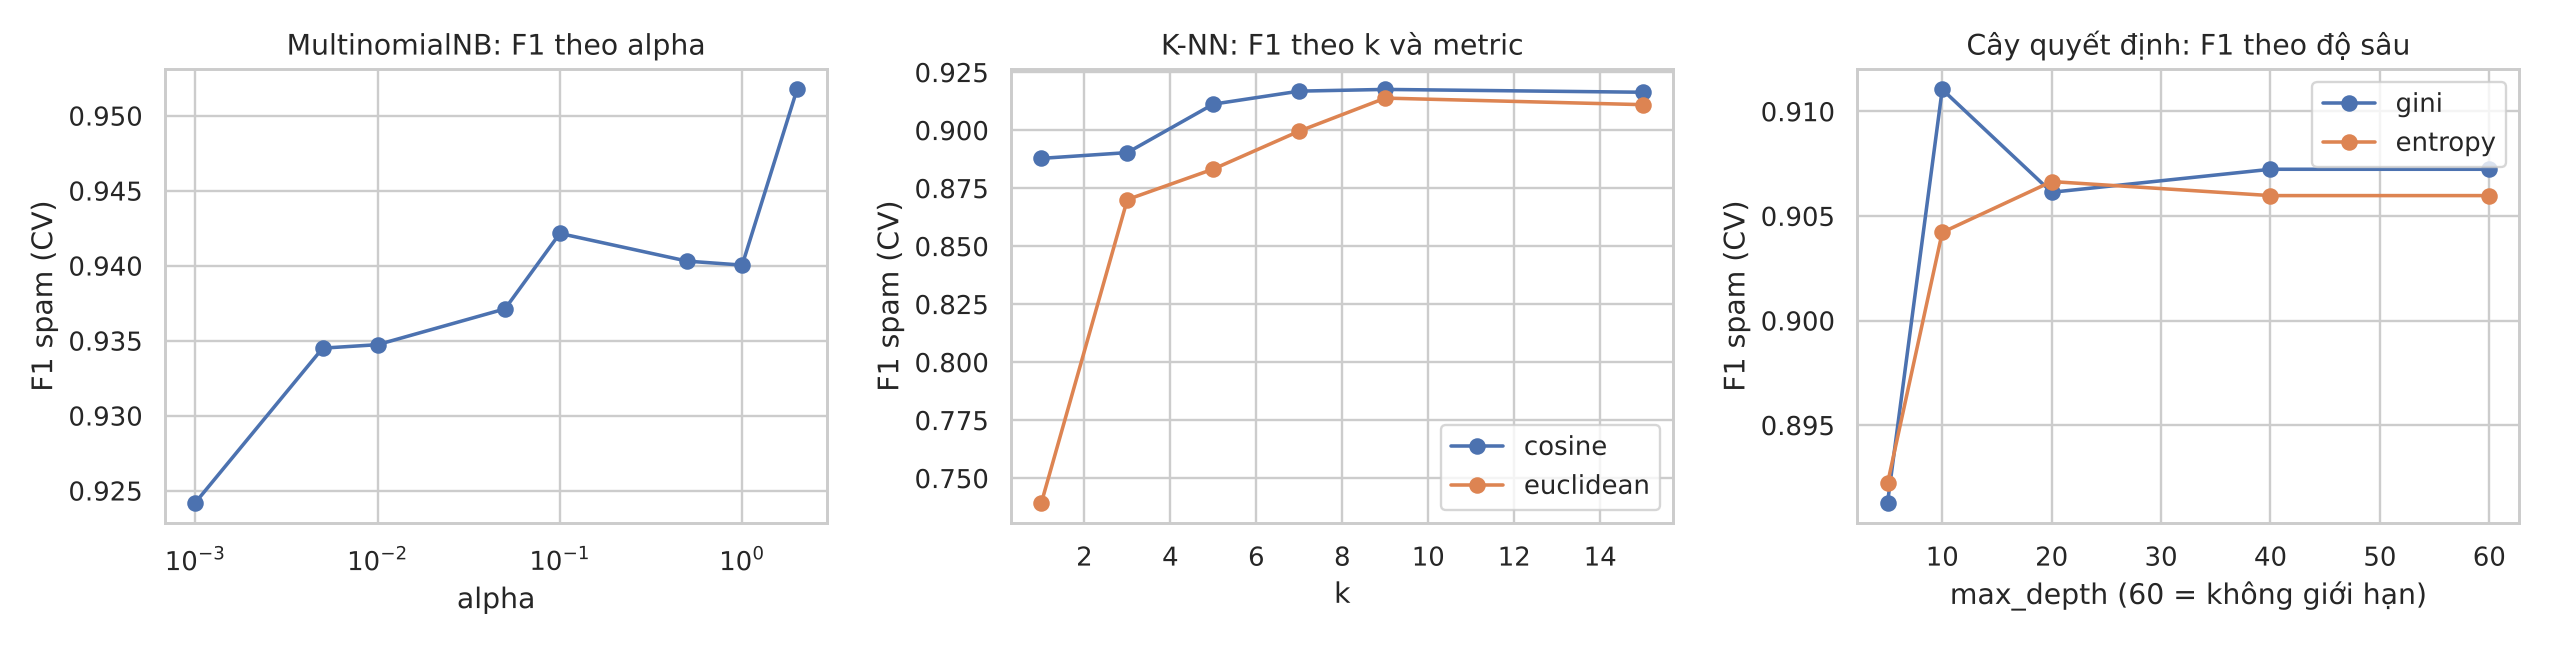
\includegraphics[width=\textwidth]{images/stage2_param_curves.png}
    \caption{Đường cong biến thiên điểm F1 CV theo siêu tham số chính: MultinomialNB theo $\alpha$ (trái), K-NN theo $K$ và metric (giữa), Cây quyết định theo độ sâu \texttt{max\_depth} (phải)}
    \label{fig:param-curves}
    \Nguon{Trích xuất tự động từ module run\_experiments.py}
\end{figure}

\begin{enumerate}
    \item \textbf{MultinomialNB theo $\alpha$ (Hình trái):} Điểm F1 CV tăng dần đều từ vùng $\alpha = 0.001$ và đạt đỉnh cực đại tại $\alpha = 2.0$. Do điểm cực đại nằm ở cận trên của lưới ban đầu, nhóm đã triển khai thêm thực nghiệm mở rộng ở Mục~\ref{sec:mo-rong-alpha}.
    \item \textbf{K-NN theo $K$ và hàm khoảng cách (Hình giữa):} Khoảng cách \texttt{cosine} thể hiện sự vượt trội hoàn toàn so với \texttt{euclidean} tại mọi giá trị $K$. Đường cong F1 của \texttt{cosine} tăng nhanh từ $K=1$ đến $K=7$ và đi vào vùng bão hòa ổn định ở $K=7, 9, 15$. Giá trị $K=9$ được lựa chọn vì mang lại sự cân bằng tốt nhất giữa độ mịn của ranh giới quyết định và khả năng kháng nhiễu.
    \item \textbf{Cây quyết định theo \texttt{max\_depth} (Hình phải):} Tiêu chí \texttt{gini} mang lại hiệu năng nhỉnh hơn tiêu chí \texttt{entropy}. Đường cong F1 đạt đỉnh rõ nét tại độ sâu \texttt{max\_depth=10} ($F_1 = 0,9110$). Khi tăng độ sâu lên $20, 40$ hoặc không giới hạn (\texttt{None}), điểm F1 giảm dần do hiện tượng quá khớp (Overfitting) trên các từ vựng cá biệt.
\end{enumerate}

\section{Thực nghiệm mở rộng: Khảo sát độ nhạy tham số làm trơn $\alpha$ của Naive Bayes}
\label{sec:mo-rong-alpha}

Do trong lưới tìm kiếm ban đầu, $\alpha = 2.0$ là giá trị lớn nhất được khảo sát và đạt điểm F1 cao nhất, một câu hỏi khoa học quan trọng được đặt ra: *“Nếu tiếp tục tăng $\alpha$ lên các giá trị lớn hơn ($3, 5, 10$), liệu hiệu năng của Naive Bayes có tiếp tục tăng hay không?”*.

Để trả lời câu hỏi này, nhóm đã xây dựng module độc lập \texttt{src/extra\_nb\_alpha\_check.py}, mở rộng dải khảo sát $\alpha \in [0.1, 0.5, 1, 2, 3, 5, 10]$ và lặp lại trên 3 seed phân chia fold thẩm định chéo khác nhau để triệt tiêu nhiễu ngẫu nhiên. Kết quả trung bình được tổng hợp tại Bảng~\ref{tab:nb-alpha-sensitivity}.

\begin{table}[H]
\centering
\caption{Khảo sát độ nhạy của Multinomial Naive Bayes theo tham số làm trơn $\alpha$ (trung bình qua 3 seed phân chia fold)}
\label{tab:nb-alpha-sensitivity}
\begin{tabular}{|c|c|c|c|l|}
\hline
\textbf{Hệ số $\alpha$} & \textbf{F1-Score} & \textbf{Precision} & \textbf{Recall} & \textbf{Nhận xét xu hướng} \\
\hline
0,1 & 0,9396 & 0,9314 & 0,9483 & Mô hình nhạy, dễ báo động nhầm \\
\hline
0,5 & 0,9390 & 0,9278 & 0,9508 & Recall cao, Precision thấp \\
\hline
1,0 & 0,9396 & 0,9315 & 0,9483 & Làm trơn Laplace chuẩn \\
\hline
\textbf{2,0} & \textbf{0,9503} & \textbf{0,9541} & \textbf{0,9470} & \textbf{Điểm cân bằng tối ưu toàn cục} \\
\hline
3,0 & 0,9488 & 0,9622 & 0,9361 & Precision tăng, Recall bắt đầu giảm \\
\hline
5,0 & 0,9460 & 0,9725 & 0,9214 & Bắt đầu bỏ sót nhiều tin rác \\
\hline
10,0 & 0,9409 & 0,9826 & 0,9029 & Precision rất cao nhưng Recall tụt sâu \\
\hline
\end{tabular}
\Nguon{Trích xuất tự động từ module extra\_nb\_alpha\_check.py}
\end{table}

\textbf{Quy luật đánh đổi sâu sắc:}
Số liệu tại Bảng~\ref{tab:nb-alpha-sensitivity} đã làm sáng tỏ bản chất toán học của hệ số làm trơn $\alpha$:
\begin{itemize}
    \item Khi $\alpha$ càng lớn, xác suất có điều kiện $\hat{P}(w_i|y)$ càng bị kéo mạnh về phía phân phối đều $\frac{1}{|\mathcal{V}|}$. Mô hình trở nên "thận trọng" và dè dặt hơn rất nhiều khi gán nhãn spam cho một tin nhắn.
    \item Do đó, khi $\alpha$ tăng từ $2.0$ lên $10.0$, chỉ số Precision tăng vọt từ $95,41\%$ lên tới \textbf{$98,26\%$} (hầu như không bao giờ chặn nhầm tin hợp lệ), nhưng phải trả giá bằng việc chỉ số Recall tụt giảm từ $94,70\%$ xuống \textbf{$90,29\%$} (bỏ lọt nhiều tin rác hơn).
    \item Điểm số F1-score đạt đỉnh thực sự tại $\alpha = 2.0$ ($F_1 = 0,9503$) và bắt đầu suy giảm đơn điệu khi $\alpha > 2.0$. Thực nghiệm này chứng minh trọn vẹn rằng $\alpha = 2.0$ là điểm tối ưu toàn cục đích thực.
\end{itemize}

\section{Thực nghiệm có kiểm soát về các tham số của Vectorizer}
\label{sec:thuc-nghiem-vectorizer}

Để đáp ứng toàn diện yêu cầu tại Mục 3.1 trong tài liệu hướng dẫn bài tập lớn của học phần (khảo sát ảnh hưởng của n-gram, \texttt{min\_df}, \texttt{max\_df} và số lượng đặc trưng), nhóm đã tiến hành một thực nghiệm có kiểm soát nghiêm ngặt thông qua module \texttt{src/vectorizer\_sensitivity.py}. Đối với mỗi mô hình, nhóm giữ nguyên tiền xử lý, loại biểu diễn và siêu tham số tối ưu đã chọn ở Bảng~\ref{tab:cau-hinh-toi-uu}, chỉ thay đổi độc lập từng tham số vector hóa trên tập huấn luyện (5-fold CV).

\begin{figure}[H]
    \centering
    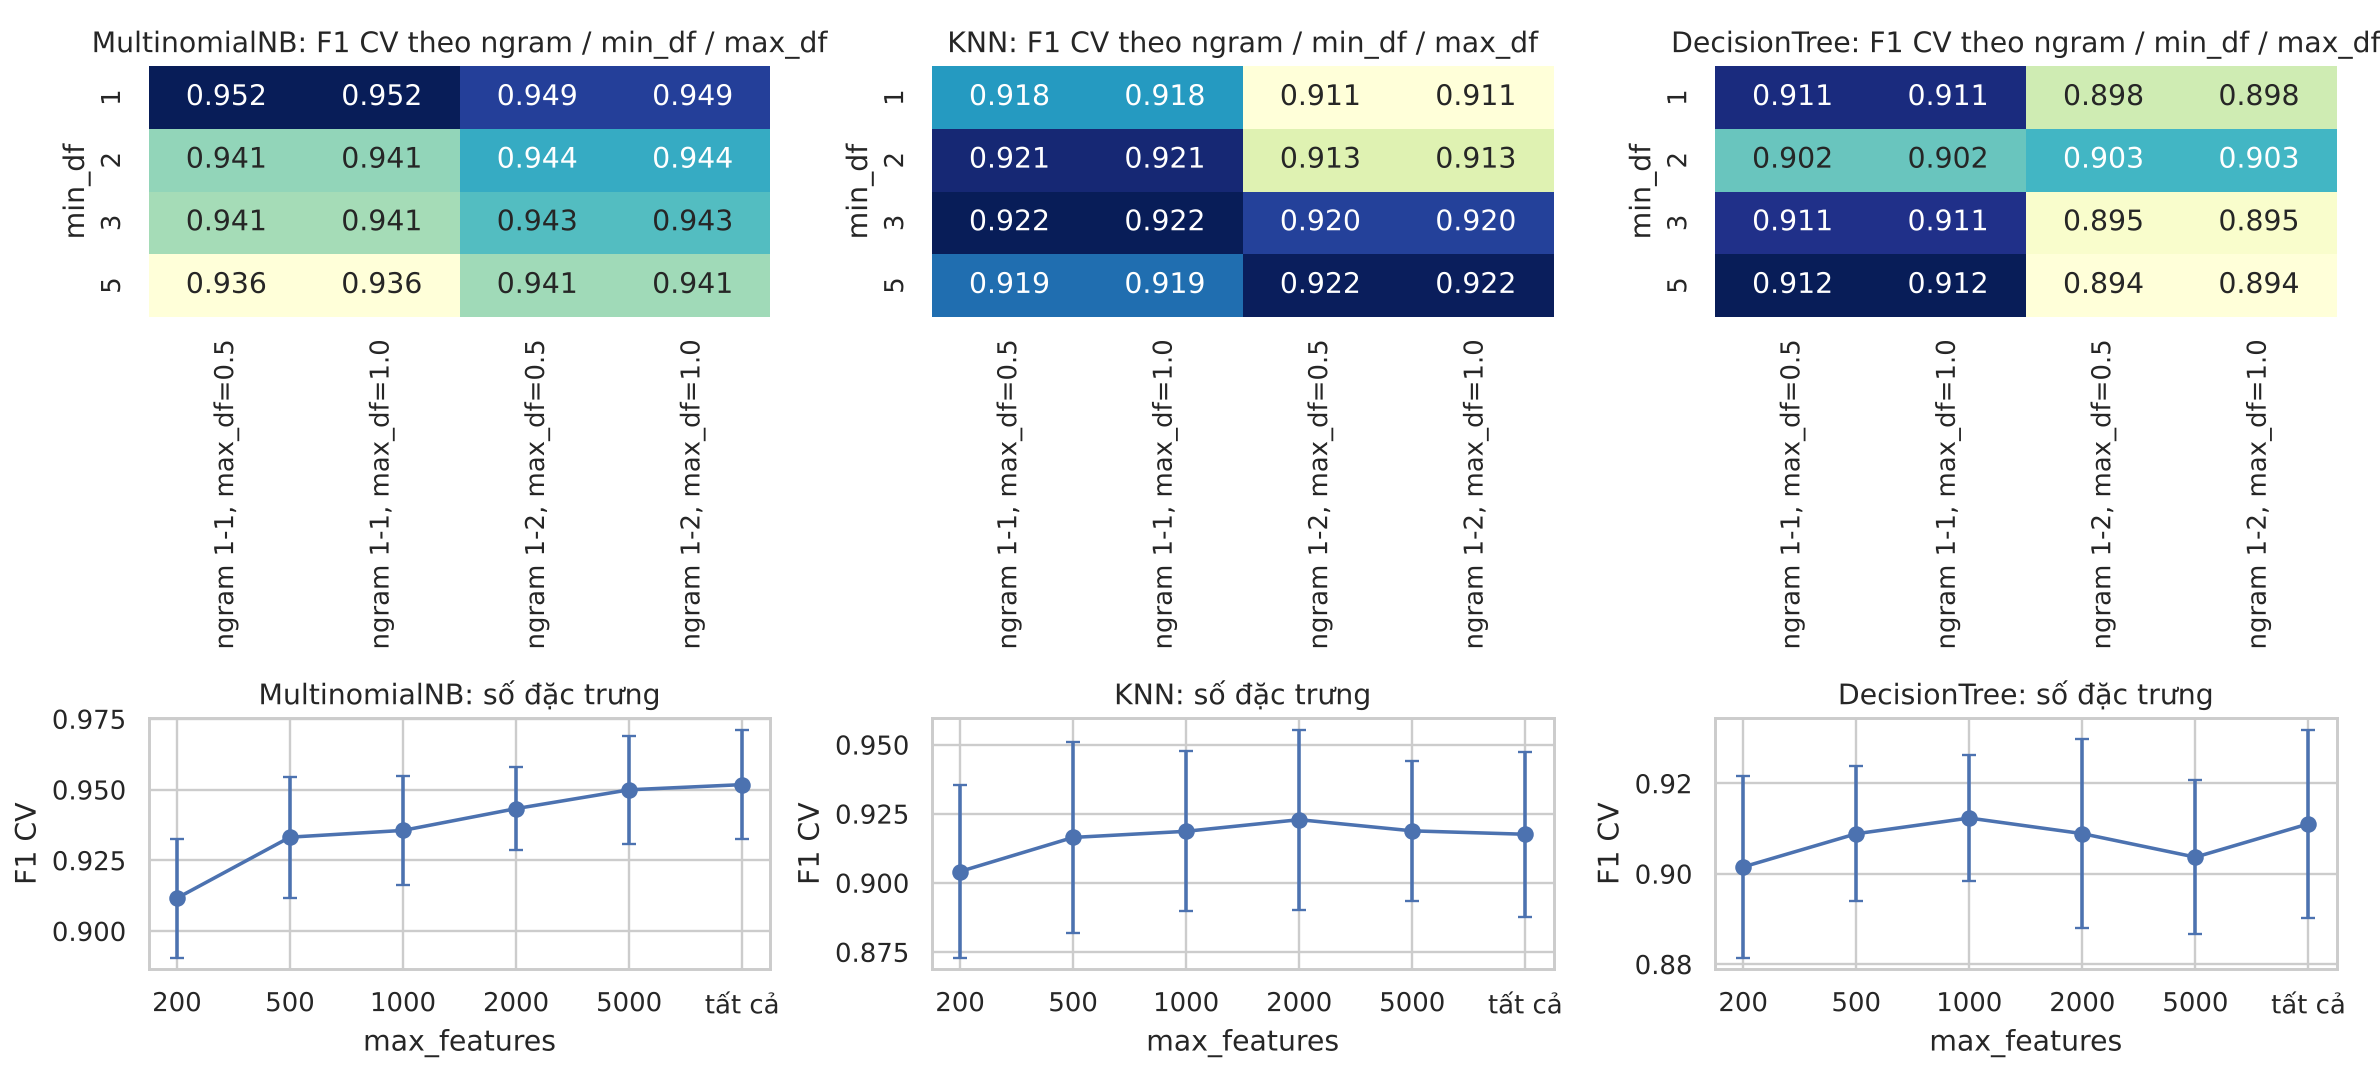
\includegraphics[width=\textwidth]{images/vectorizer_sensitivity.png}
    \caption{Thực nghiệm có kiểm soát về tham số Vectorizer: Lưới n-gram $\times$ \texttt{min\_df} $\times$ \texttt{max\_df} (hàng trên) và đường cong F1 theo số lượng đặc trưng \texttt{max\_features} (hàng dưới)}
    \label{fig:vectorizer-sensitivity}
    \Nguon{Trích xuất tự động từ module vectorizer\_sensitivity.py}
\end{figure}

\subsection{Khảo sát tương tác n-gram, \texttt{min\_df} và \texttt{max\_df}}
Bảng~\ref{tab:vectorizer-grid} trình bày chi tiết điểm F1 CV của 3 mô hình khi thay đổi bậc n-gram và ngưỡng tần số tài liệu tối thiểu \texttt{min\_df} (khi \texttt{max\_df=1.0}).

\begin{table}[H]
\centering
\caption{F1 CV theo bậc n-gram và ngưỡng min\_df (với max\_df=1.0)}
\label{tab:vectorizer-grid}
\begin{tabular}{|l|l|c|c|c|c|}
\hline
\textbf{Mô hình} & \textbf{Biểu diễn n-gram} & \textbf{min\_df=1} & \textbf{min\_df=2} & \textbf{min\_df=3} & \textbf{min\_df=5} \\
\hline
\multirow{2}{*}{\textbf{MultinomialNB}} & unigram (1-1) & \textbf{0,9518} & 0,9412 & 0,9407 & 0,9357 \\
\cline{2-6}
& unigram + bigram (1-2) & 0,9492 & 0,9443 & 0,9432 & 0,9408 \\
\hline
\multirow{2}{*}{\textbf{K-NN}} & unigram (1-1) & 0,9176 & 0,9213 & \textbf{0,9219} & 0,9188 \\
\cline{2-6}
& unigram + bigram (1-2) & 0,9112 & 0,9130 & 0,9201 & 0,9218 \\
\hline
\multirow{2}{*}{\textbf{DecisionTree}} & unigram (1-1) & 0,9110 & 0,9020 & 0,9106 & \textbf{0,9125} \\
\cline{2-6}
& unigram + bigram (1-2) & 0,8985 & 0,9034 & 0,8952 & 0,8944 \\
\hline
\end{tabular}
\Nguon{Trích xuất tự động từ results/vectorizer\_sensitivity.csv}
\end{table}

\textbf{Các quan sát thực nghiệm cốt lõi:}
\begin{enumerate}
    \item \textbf{Về tham số \texttt{max\_df}:} Khi chuyển từ \texttt{max\_df=1.0} sang \texttt{max\_df=0.5}, kết quả F1 CV của toàn bộ các ô ở cả ba mô hình \textbf{hoàn toàn giống hệt nhau} (sai số $0.0000$). Điều này chứng minh rằng trong tập dữ liệu SMS Spam, không có bất kỳ từ khóa nào xuất hiện trong hơn 50\% tổng số tin nhắn. Do đó, tham số \texttt{max\_df} không có tác động thực tế trong bài toán này.
    \item \textbf{Về vai trò của Bigram và kiểm chứng Giả thuyết H2:} Khi so sánh công bằng ở cùng ngưỡng \texttt{min\_df=2}, mô hình kết hợp unigram + bigram của Naive Bayes đạt F1 là $0,9443$, chỉ nhỉnh hơn unigram ($0,9412$) một lượng rất nhỏ $0,0031$. Tuy nhiên, độ lệch chuẩn F1 giữa các fold của Naive Bayes là $\approx 0,017$. Do mức chênh lệch nhỏ hơn nhiều so với độ lệch chuẩn, \textbf{Giả thuyết H2 không được dữ liệu thực nghiệm ủng hộ}. Trong các tin nhắn SMS rất ngắn, các cụm hai từ hiếm khi lặp lại đủ nhiều để tạo ra sự đột phá ngữ nghĩa so với các từ đơn lẻ.
    \item \textbf{Về ngưỡng \texttt{min\_df}:} Việc tăng \texttt{min\_df} từ 1 lên 5 giúp loại bỏ hàng nghìn từ hiếm, giảm kích thước từ vựng nhưng làm điểm F1 của Naive Bayes giảm nhẹ từ $0,9518$ xuống $0,9357$.
\end{enumerate}

\subsection{Khảo sát giới hạn số lượng đặc trưng (\texttt{max\_features})}
Bảng~\ref{tab:max-features-study} thể hiện sự biến thiên của F1 CV khi giới hạn kích thước từ vựng tối đa từ 200 từ đến toàn bộ từ điển ($\approx 6.500$ từ).

\begin{table}[H]
\centering
\caption{F1 CV theo số lượng đặc trưng tối đa max\_features (unigram, min\_df=1)}
\label{tab:max-features-study}
\begin{tabular}{|l|c|c|c|c|c|c|}
\hline
\textbf{Mô hình} & \textbf{200 từ} & \textbf{500 từ} & \textbf{1.000 từ} & \textbf{2.000 từ} & \textbf{5.000 từ} & \textbf{Tất cả ($\approx$6.500)} \\
\hline
MultinomialNB & 0,9116 & 0,9332 & 0,9356 & 0,9433 & 0,9499 & \textbf{0,9518} \\
\hline
K-NN & 0,9041 & 0,9164 & 0,9187 & \textbf{0,9229} & 0,9188 & 0,9176 \\
\hline
DecisionTree & 0,9015 & 0,9089 & \textbf{0,9123} & 0,9089 & 0,9037 & 0,9110 \\
\hline
\end{tabular}
\Nguon{Trích xuất tự động từ results/vectorizer\_sensitivity.csv}
\end{table}

Từ Bảng~\ref{tab:max-features-study} và biểu đồ hàng dưới tại Hình~\ref{fig:vectorizer-sensitivity}:
\begin{itemize}
    \item Chỉ khi cắt giảm từ điển xuống mức cực đoan (200 từ), hiệu năng mô hình mới bị suy giảm rõ rệt (F1 của Naive Bayes giảm từ $0,9518$ xuống $0,9116$, mức giảm gấp 2 lần độ lệch chuẩn).
    \item Từ ngưỡng \textbf{2.000 từ} trở lên, hiệu năng của cả 3 mô hình đã tiệm cận mức tối đa và đi vào vùng bão hòa hoàn toàn.
    \item Với tài nguyên tính toán hiện đại, việc lưu trữ 6.500 đặc trưng là hoàn toàn khả thi và không gây áp lực bộ nhớ, do đó giữ lại toàn bộ từ vựng là giải pháp tối ưu.
\end{itemize}

\section{Đánh giá tổng hợp trên tập kiểm thử độc lập (Test Set)}
\label{sec:danh-gia-test}

Sau khi đã xác định được cấu hình tối ưu nhất cho từng thuật toán thông qua quy trình thẩm định chéo nghiêm ngặt trên tập huấn luyện, toàn bộ 3 mô hình được huấn luyện lại trên toàn bộ 4.136 mẫu của tập Train và được đánh giá một lần duy nhất trên tập kiểm thử độc lập gồm 1.035 mẫu (trong đó có 131 mẫu tin nhắn rác).

\subsection{Đối sánh toàn diện Baseline và Mô hình tinh chỉnh}
Bảng~\ref{tab:baseline-vs-tuned} đối sánh chi tiết sự cải thiện của từng chỉ số giữa phương án Baseline ban đầu và mô hình sau tinh chỉnh tối ưu.

\begin{table}[H]
\centering
\caption{Đối sánh hiệu năng giữa phương án Baseline và Cấu hình tinh chỉnh trên tập kiểm thử}
\label{tab:baseline-vs-tuned}
\begin{tabular}{|l|l|c|c|c|c|}
\hline
\textbf{Thuật toán} & \textbf{Phương án} & \textbf{Accuracy} & \textbf{Precision} & \textbf{Recall} & \textbf{F1-Score} \\
\hline
\multirow{2}{*}{\textbf{Multinomial NB}} & Baseline & 0,9807 & 0,9512 & 0,8931 & 0,9213 \\
\cline{2-6}
& Tinh chỉnh & \textbf{0,9913} & \textbf{0,9766} & \textbf{0,9542} & \textbf{0,9653} \\
\hline
\multirow{2}{*}{\textbf{K-NN}} & Baseline & 0,9072 & 1,0000 & 0,2672 & 0,4217 \\
\cline{2-6}
& Tinh chỉnh & \textbf{0,9826} & \textbf{0,9593} & \textbf{0,9008} & \textbf{0,9291} \\
\hline
\multirow{2}{*}{\textbf{Decision Tree}} & Baseline & 0,9691 & 0,9024 & 0,8473 & 0,8740 \\
\cline{2-6}
& Tinh chỉnh & \textbf{0,9874} & \textbf{1,0000} & \textbf{0,9008} & \textbf{0,9478} \\
\hline
\end{tabular}
\Nguon{Trích xuất từ results/baseline\_vs\_tuned.csv}
\end{table}

Kết quả ở Bảng~\ref{tab:baseline-vs-tuned} chứng minh sự tiến bộ vượt bậc của toàn bộ các mô hình sau khi được tối ưu hóa:
\begin{itemize}
    \item Multinomial Naive Bayes nâng F1 từ $0,9213$ lên \textbf{$0,9653$} (Recall tăng ấn tượng từ $89,31\%$ lên $95,42\%$).
    \item K-NN tạo ra bước nhảy vọt ngoạn mục nhất: F1 tăng từ $0,4217$ lên \textbf{$0,9291$} (Recall tăng từ $26,72\%$ lên $90,08\%$, khắc phục hoàn toàn nhược điểm bỏ sót tin rác).
    \item Cây quyết định nâng F1 từ $0,8740$ lên \textbf{$0,9478$}, đặc biệt đạt được chỉ số \textbf{Precision tuyệt đối $100\%$} (không chặn nhầm bất kỳ tin nhắn hợp lệ nào trên tập test).
\end{itemize}

\subsection{Bảng chỉ số đánh giá cuối cùng}
Bảng~\ref{tab:ket-qua-cuoi-cung} tổng hợp toàn bộ các chỉ số kiểm thử cuối cùng cùng số lượng lỗi thực tế tương ứng của 3 mô hình.

\begin{table}[H]
\centering
\caption{Kết quả đánh giá kiểm thử cuối cùng trên tập Test (1.035 tin nhắn, 131 spam)}
\label{tab:ket-qua-cuoi-cung}
\begin{tabular}{|l|c|c|c|c|c|c|}
\hline
\textbf{Mô hình tối ưu} & \textbf{Accuracy} & \textbf{Precision} & \textbf{Recall} & \textbf{F1-Score} & \textbf{ROC-AUC} & \textbf{Số lỗi (FP / FN)} \\
\hline
\textbf{Multinomial NB} & \textbf{0,9913} & 0,9766 & \textbf{0,9542} & \textbf{0,9653} & 0,9860 & \textbf{3 / 6 (Tổng: 9)} \\
\hline
\textbf{K-NN} & 0,9826 & 0,9593 & 0,9008 & 0,9291 & \textbf{0,9919} & 5 / 13 (Tổng: 18) \\
\hline
\textbf{Decision Tree} & 0,9874 & \textbf{1,0000} & 0,9008 & 0,9478 & 0,9500 & \textbf{0 / 13 (Tổng: 13)} \\
\hline
\end{tabular}
\Nguon{Trích xuất từ results/final\_test\_results.csv và summary.json}
\end{table}

\subsection{Trực quan hóa Ma trận nhầm lẫn và Đường cong ROC}
Hình~\ref{fig:confusion-matrices} thể hiện ma trận nhầm lẫn trực quan của 3 mô hình trên tập kiểm thử 1.035 mẫu.

\begin{figure}[H]
    \centering
    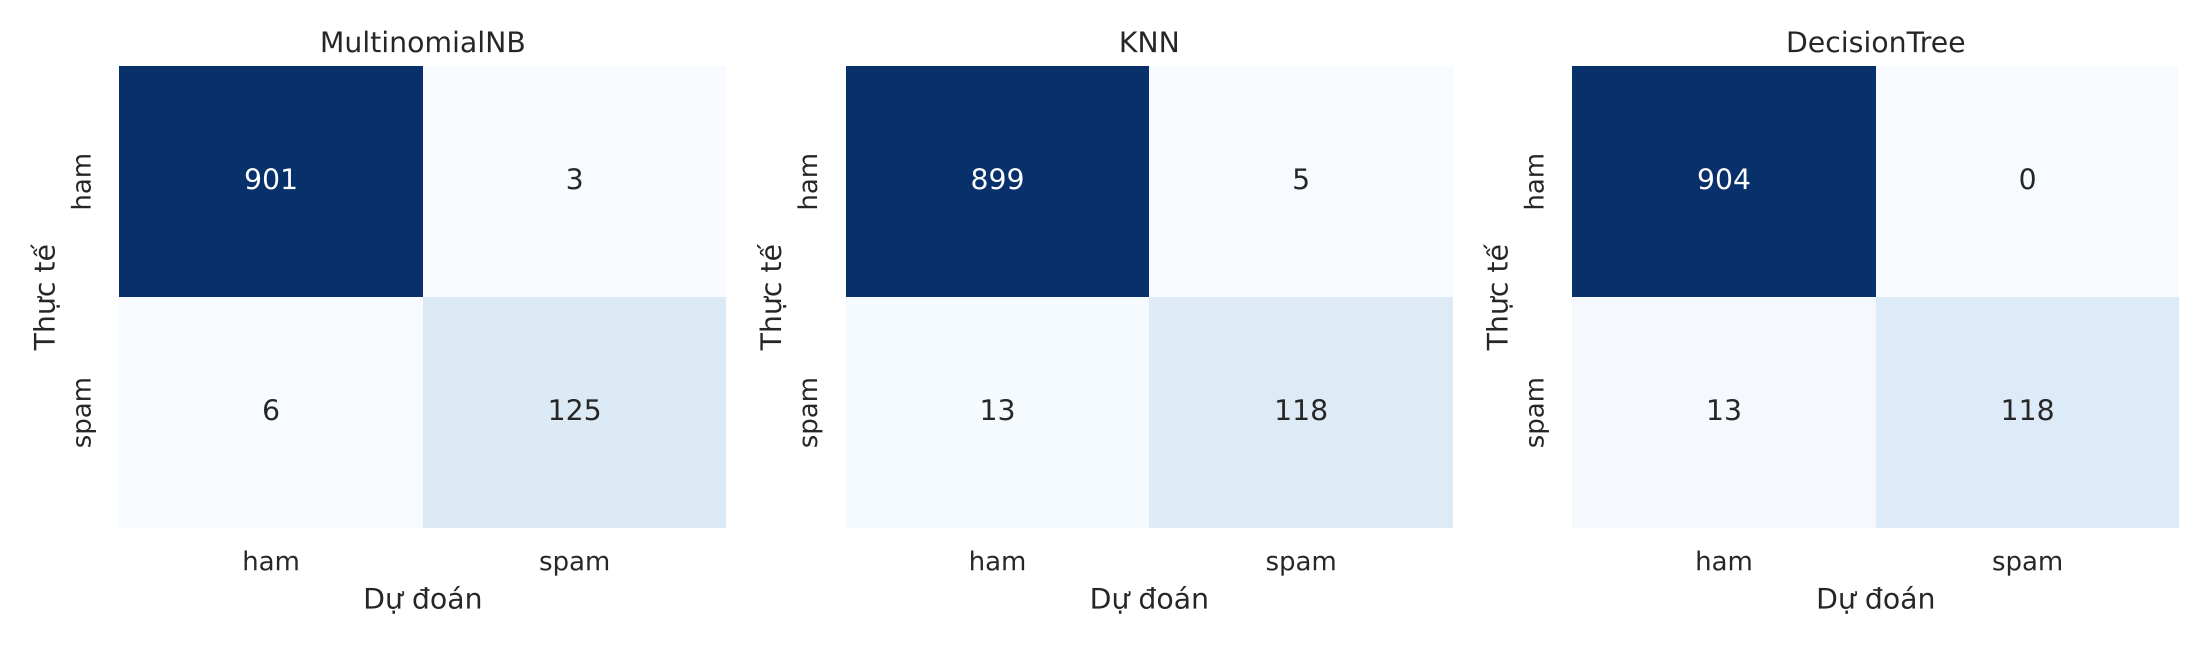
\includegraphics[width=\textwidth]{images/confusion_matrices.png}
    \caption{Ma trận nhầm lẫn của 3 mô hình tối ưu trên tập kiểm thử (1.035 tin nhắn)}
    \label{fig:confusion-matrices}
    \Nguon{Trích xuất tự động từ module run\_experiments.py}
\end{figure}

Từ ma trận nhầm lẫn tại Hình~\ref{fig:confusion-matrices}:
\begin{itemize}
    \item \textbf{MultinomialNB:} Dự đoán chính xác 901/904 tin hợp lệ và 125/131 tin nhắn rác. Chỉ có đúng 3 trường hợp báo nhầm (FP) và 6 trường hợp bỏ sót (FN), đạt tổng số lỗi thấp nhất toàn hệ thống (9 lỗi / 1.035 tin).
    \item \textbf{K-NN:} Dự đoán chính xác 899/904 tin hợp lệ và 118/131 tin rác. Có 5 trường hợp báo nhầm (FP) và 13 trường hợp bỏ sót (FN).
    \item \textbf{Decision Tree:} Đạt thành tích đặc biệt khi dự đoán hoàn hảo 904/904 tin hợp lệ ($0$ trường hợp báo nhầm FP), nhưng bỏ sót 13 tin nhắn rác (FN).
\end{itemize}

\begin{figure}[H]
    \centering
    \begin{minipage}{0.48\textwidth}
        \centering
        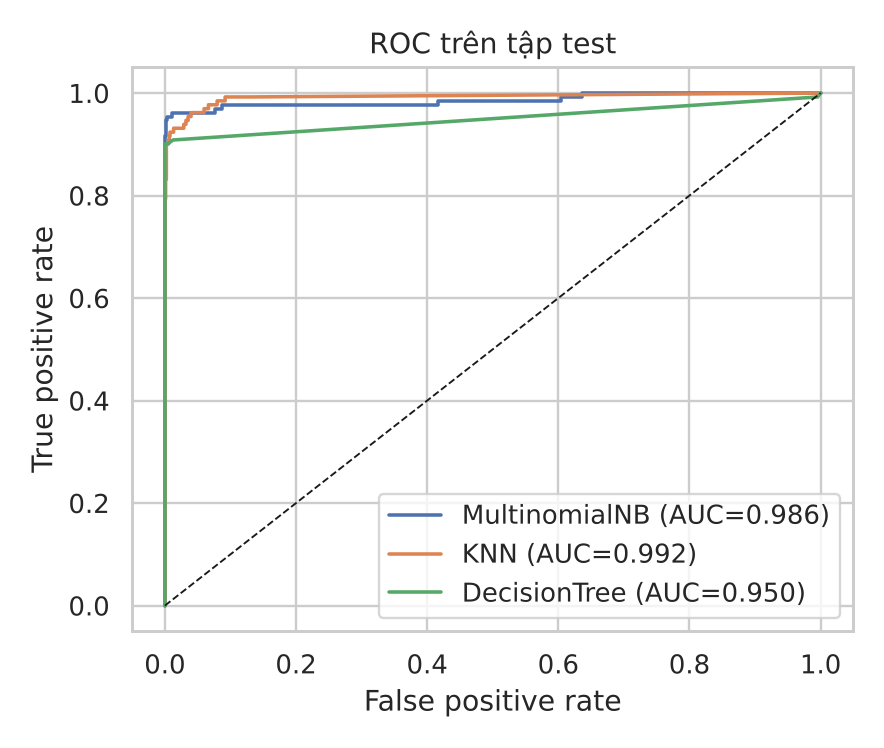
\includegraphics[width=\textwidth]{images/roc_curves.png}
        \caption*{(a) Đường cong ROC trên tập kiểm thử}
    \end{minipage}
    \hfill
    \begin{minipage}{0.50\textwidth}
        \centering
        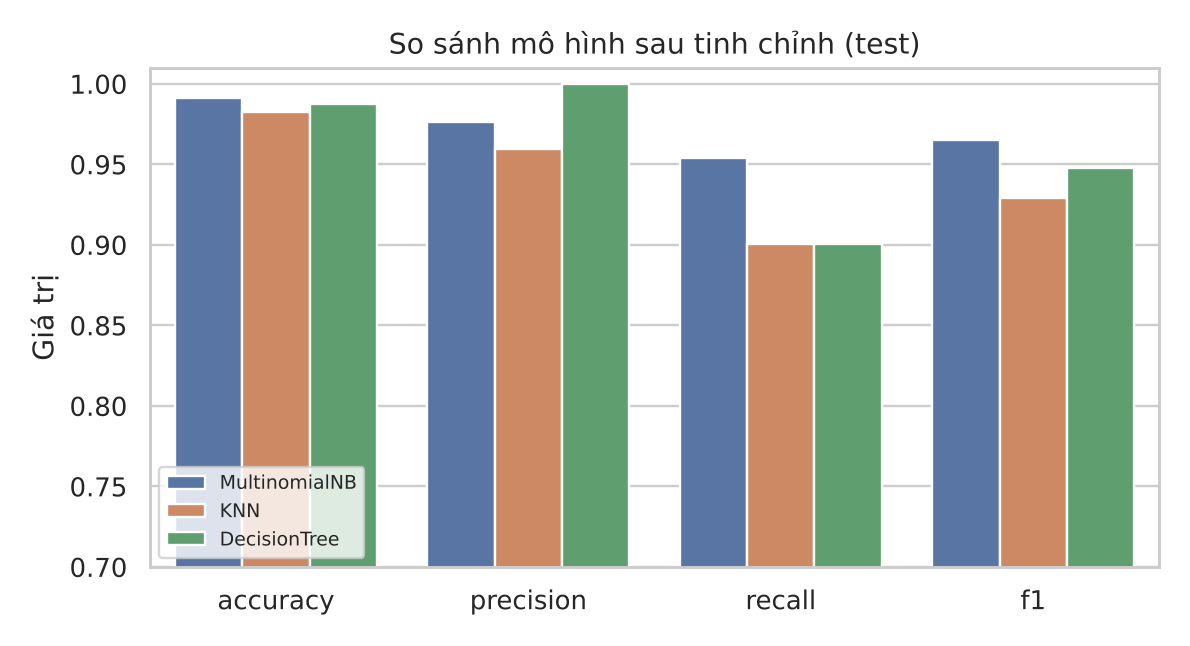
\includegraphics[width=\textwidth]{images/final_metric_bars.png}
        \caption*{(b) Biểu đồ cột đối sánh các độ đo}
    \end{minipage}
    \caption{Đường cong ROC và biểu đồ cột đối sánh các chỉ số hiệu năng của 3 mô hình tối ưu}
    \label{fig:roc-and-bars}
    \Nguon{Trích xuất tự động từ module run\_experiments.py}
\end{figure}

Hình~\ref{fig:roc-and-bars}a thể hiện đường cong ROC của cả 3 mô hình đều áp sát góc trên bên trái, minh chứng cho năng lực phân loại vượt trội. Đáng chú ý, mô hình \textbf{K-NN đạt chỉ số ROC-AUC cao nhất hệ thống lên tới $0,9919$}, vượt qua cả Naive Bayes ($0,9860$) và Cây quyết định ($0,9500$). Điều này chứng tỏ K-NN có khả năng xếp hạng xác suất (Probability Ranking) cực tốt; lý do điểm F1 của K-NN thấp hơn Naive Bayes là do ngưỡng cắt xác suất mặc định $\tau = 0.5$ chưa phải là ngưỡng tối ưu nhất đối với lớp thiểu số.

\section{Phân tích độ ổn định qua 5 lần phân chia ngẫu nhiên (5-Seed Stability Analysis)}
\label{sec:do-on-dinh-seed}

Một điểm yếu cố hữu của việc đánh giá mô hình chỉ trên một lần phân chia Train/Test duy nhất là sự phụ thuộc vào tính ngẫu nhiên: tập kiểm thử chỉ chứa 131 mẫu tin nhắn rác, do đó việc sai khác chỉ 1 tin nhắn spam duy nhất đã làm thay đổi chỉ số Recall tới gần \textbf{$0,8$ điểm phần trăm} ($\frac{1}{131} \approx 0,763\%$).

Để kiểm chứng tính vững chắc (Robustness) và loại bỏ yếu tố may rủi của một lần chia dữ liệu cụ thể, nhóm đã tiến hành thực nghiệm kiểm tra độ ổn định: giữ cố định toàn bộ siêu tham số tối ưu đã chọn ở Bảng~\ref{tab:cau-hinh-toi-uu}, lặp lại quy trình phân chia Stratified 80/20 trên \textbf{5 giá trị mầm ngẫu nhiên khác nhau} (\texttt{random\_state} $\in \{0, 1, 2, 3, 4\}$). Kết quả trung bình và độ lệch chuẩn ($\text{Mean} \pm \text{Std}$) được tổng hợp tại Bảng~\ref{tab:seed-stability}.

\begin{table}[H]
\centering
\caption{Độ ổn định hiệu năng của các mô hình qua 5 lần phân chia Train/Test khác nhau}
\label{tab:seed-stability}
\begin{tabular}{|l|c|c|c|c|c|}
\hline
\textbf{Mô hình} & \textbf{Accuracy} & \textbf{Precision} & \textbf{Recall} & \textbf{F1-Score} & \textbf{ROC-AUC} \\
\hline
\textbf{MultinomialNB} & $0,9865 \pm 0,0050$ & $0,9470 \pm 0,0280$ & $\mathbf{0,9466 \pm 0,0179}$ & $\mathbf{0,9467 \pm 0,0195}$ & $\mathbf{0,9879 \pm 0,0053}$ \\
\hline
\textbf{K-NN} & $\mathbf{0,9838 \pm 0,0032}$ & $\mathbf{0,9662 \pm 0,0129}$ & $0,9038 \pm 0,0368$ & $0,9335 \pm 0,0147$ & $0,9809 \pm 0,0045$ \\
\hline
\textbf{DecisionTree} & $0,9778 \pm 0,0040$ & $0,9611 \pm 0,0214$ & $0,8595 \pm 0,0257$ & $0,9073 \pm 0,0175$ & $0,9450 \pm 0,0146$ \\
\hline
\end{tabular}
\Nguon{Trích xuất từ results/seed\_stability\_summary.csv}
\end{table}

\textbf{Đánh giá ý nghĩa thống kê từ Bảng~\ref{tab:seed-stability}:}
\begin{enumerate}
    \item \textbf{Multinomial Naive Bayes duy trì vị trí dẫn đầu toàn diện:} Điểm F1 trung bình đạt $0,9467$, chỉ số Recall đạt $94,66\%$ và ROC-AUC đạt $0,9879$. Đặc biệt, độ lệch chuẩn rất nhỏ ($\pm 0,0195$) chứng tỏ mô hình có tính ổn định cực cao trên các tập dữ liệu khác nhau.
    \item \textbf{So sánh Naive Bayes và Cây quyết định:} Mức chênh lệch điểm F1 trung bình giữa Naive Bayes ($0,9467$) và Cây quyết định ($0,9073$) là \textbf{$0,0394$} (gần 4 điểm phần trăm). Mức chênh lệch này lớn hơn gấp hơn 2 lần độ lệch chuẩn ($\approx 0,018$), cho phép khẳng định với độ tin cậy thống kê cao rằng \textbf{Multinomial Naive Bayes thực sự vượt trội hơn Cây quyết định} trong bài toán phân loại tin nhắn rác.
    \item \textbf{So sánh Naive Bayes và K-NN:} Mức chênh lệch điểm F1 trung bình giữa Naive Bayes ($0,9467$) và K-NN ($0,9335$) là \textbf{$0,0132$}. Mức chênh lệch này nhỏ hơn độ lệch chuẩn của cả hai mô hình ($0,0195$ và $0,0147$). Do đó, dưới góc độ thống kê học chặt chẽ, nhóm kết luận rằng \textbf{chưa đủ bằng chứng để khẳng định Naive Bayes vượt trội tuyệt đối so với K-NN}; cả hai mô hình đều có hiệu năng tiệm cận và bổ trợ rất tốt cho nhau.
\end{enumerate}

\section{Đánh giá hiệu năng thời gian và độ phức tạp tính toán}
\label{sec:hieu-nang-thoi-gian}

Bên cạnh các chỉ số chất lượng phân loại, chi phí tính toán và thời gian đáp ứng thời gian thực (Latency) là yếu tố quyết định tính khả thi khi triển khai mô hình vào hệ thống gateway viễn thông.

Bảng~\ref{tab:thoi-gian-tinh-toan} tổng hợp số lượng đặc trưng và thời gian thực thi dự đoán cho toàn bộ 1.035 tin nhắn của tập kiểm thử trên cùng một lõi CPU.

\begin{table}[H]
\centering
\caption{Số lượng đặc trưng và thời gian dự đoán trên tập kiểm thử (1.035 tin nhắn)}
\label{tab:thoi-gian-tinh-toan}
\begin{tabular}{|l|c|c|c|}
\hline
\textbf{Thuật toán} & \textbf{Số lượng đặc trưng} & \textbf{Thời gian dự đoán (giây)} & \textbf{Tốc độ (tin nhắn / giây)} \\
\hline
\textbf{Multinomial Naive Bayes} & 6.516 từ vựng & \textbf{0,0371} giây & $\approx 27.900$ tin/giây \\
\hline
\textbf{Cây quyết định (Decision Tree)} & 6.516 từ vựng & \textbf{0,0371} giây & $\approx 27.900$ tin/giây \\
\hline
\textbf{K-Láng giềng gần nhất (K-NN)} & 6.782 từ vựng & \textbf{0,1190} giây & $\approx 8.700$ tin/giây \\
\hline
\end{tabular}
\Nguon{Trích xuất tự động từ results/summary.json}
\end{table}

\textbf{Nhận xét về độ phức tạp thuật toán:}
\begin{itemize}
    \item \textbf{Multinomial Naive Bayes và Cây quyết định} có thời gian dự đoán cực kỳ nhanh ($0,0371$ giây cho 1.035 tin, tương đương chưa đầy 36 microgiây cho mỗi tin nhắn). Quá trình dự đoán của Naive Bayes chỉ bao gồm phép nhân vector thưa và cộng logarit xác suất $O(d)$, trong khi Cây quyết định chỉ duyệt qua tối đa 10 tầng so sánh nhị phân $O(\text{depth})$. Cả hai mô hình đều hoàn toàn đáp ứng yêu cầu xử lý thời gian thực tải cao.
    \item \textbf{K-NN} có thời gian dự đoán chậm hơn tới \textbf{3,2 lần} ($0,1190$ giây). Do bản chất là thuật toán học lười (Lazy Learning), K-NN bắt buộc phải lưu toàn bộ 4.136 vector huấn luyện vào bộ nhớ và thực hiện phép nhân vô hướng tính khoảng cách Cosine với toàn bộ tập mẫu mỗi khi có một tin nhắn mới cần phân loại ($O(N \cdot d)$). Điều này khiến K-NN gặp rào cản lớn về tài nguyên khi mở rộng quy mô dữ liệu lên hàng triệu người dùng.
\end{itemize}

\section{Tóm tắt chương 4}
Chương 4 đã phản ánh một bức tranh thực nghiệm quy mô lớn và toàn diện. Từ phương án Baseline ban đầu với sự thất bại của K-NN ($F_1 = 0,4217$), quy trình tối ưu hóa 2 giai đoạn đã nâng tầm hiệu năng của cả 3 mô hình lên mức xuất sắc trên tập kiểm thử độc lập: MultinomialNB đạt F1 $0,9653$, Cây quyết định đạt Precision tuyệt đối $1,000$ (F1 $0,9478$), và K-NN đạt ROC-AUC ấn tượng $0,9919$ (F1 $0,9291$). Thực nghiệm mở rộng đã xác nhận $\alpha = 2.0$ là điểm tối ưu toàn cục của Naive Bayes. Khảo sát Vectorizer có kiểm soát đã chỉ ra rằng bigram không mang lại sự khác biệt đáng kể và 2.000 từ vựng là đủ để mô hình bão hòa. Kiểm tra độ ổn định qua 5 seed đã khẳng định tính vững chắc và ưu thế vượt trội của Naive Bayes về cả độ chính xác lẫn tốc độ tính toán. Toàn bộ các ca lỗi dự đoán sẽ được mổ xẻ chi tiết trong Chương 5.